
\documentclass[journal]{IEEEtran}
%
% If IEEEtran.cls has not been installed into the LaTeX system files,
% manually specify the path to it like:
%\documentclass[journal]{./ieeetrans_template/IEEEtran}


% *** GRAPHICS RELATED PACKAGES ***
%
\ifCLASSINFOpdf
  \usepackage[pdftex]{graphicx}
  % declare the path(s) where your graphic files are
  % \graphicspath{{../pdf/}{../jpeg/}}
  % and their extensions so you won't have to specify these with
  % every instance of \includegraphics
  % \DeclareGraphicsExtensions{.pdf,.jpeg,.png}
\else
  % or other class option (dvipsone, dvipdf, if not using dvips). graphicx
  % will default to the driver specified in the system graphics.cfg if no
  % driver is specified.
  \usepackage[dvips]{graphicx}
  % declare the path(s) where your graphic files are
  % \graphicspath{{../eps/}}
  % and their extensions so you won't have to specify these with
  % every instance of \includegraphics
  % \DeclareGraphicsExtensions{.eps}
\fi
% graphicx was written by David Carlisle and Sebastian Rahtz. It is
% required if you want graphics, photos, etc. graphicx.sty is already
% installed on most LaTeX systems. The latest version and documentation can
% be obtained at: 
% http://www.ctan.org/tex-archive/macros/latex/required/graphics/
% Another good source of documentation is "Using Imported Graphics in
% LaTeX2e" by Keith Reckdahl which can be found as epslatex.ps or
% epslatex.pdf at: http://www.ctan.org/tex-archive/info/
%
% latex, and pdflatex in dvi mode, support graphics in encapsulated
% postscript (.eps) format. pdflatex in pdf mode supports graphics
% in .pdf, .jpeg, .png and .mps (metapost) formats. Users should ensure
% that all non-photo figures use a vector format (.eps, .pdf, .mps) and
% not a bitmapped formats (.jpeg, .png). IEEE frowns on bitmapped formats
% which can result in "jaggedy"/blurry rendering of lines and letters as
% well as large increases in file sizes.
%
% You can find documentation about the pdfTeX application at:
% http://www.tug.org/applications/pdftex


% *** Do not adjust lengths that control margins, column widths, etc. ***
% *** Do not use packages that alter fonts (such as pslatex).         ***
% There should be no need to do such things with IEEEtran.cls V1.6 and later.
% (Unless specifically asked to do so by the journal or conference you plan
% to submit to, of course. )

% correct bad hyphenation here
\hyphenation{op-tical net-works semi-conduc-tor}


\begin{document}

% paper title
% can use linebreaks \\ within to get better formatting as desired
\title{Adaptive MIMO Decoder \\ {\Large EE290C Project Final Report}}

% use \thanks{} to gain access to the first footnote area
% a separate \thanks must be used for each paragraph as LaTeX2e's \thanks
% was not built to handle multiple paragraphs
%

\author{Antonio Puglielli and Simon Scott}


% make the title area
\maketitle

%%%% OBJECTIVES SECTION %%%%
\section{Objectives}

\IEEEPARstart{M}{IMO} refers to the use of multiple transmit antennas {\em and} multiple receive antennas to spatially multiplex data streams over a channel, as illustrated in Figure~\ref{mimo_cartoon}. This channel is often represented by a complex matrix ({\em H}), and can change over time. Although MIMO can be used to increase reliability of a link, this project is only concerned with the use of MIMO to improve throughput. Furthermore, only the single user case will be considered, meaning that all the receive antennas are assumed to be on the same hardware and can share information.

The objectives of this project are therefore to develop a VLSI implementation of a MIMO decoder that:
\begin{itemize}
\item supports the antenna configurations and modulation schemes used in both 802.11ac and LTE.
\item meets both the 802.11ac and LTE throughput requirements.
\item is able to adapt to changing channel conditions.
\item is both compile-time and run-time configurable.
\end{itemize}

\begin{figure}[!h]
\centering
\includegraphics*[width=5cm, viewport = 300 0 560 130]{images/agilent_mimo.jpg}
\caption{A 2x2 MIMO configuration}
\label{mimo_cartoon}
\end{figure}


%%%% MOTIVATION AND ALGORITHM SECTION %%%%
\section{Algorithm Evaluation and Selection}
\label{matlab_comparison_section}

The two main classes of MIMO detection algorithms are those of linear and nonlinear algorithms. Linear detection algorithms refer to techniques which form the detected symbols as a linear combination of the received data. Nonlinear detection schemes are more complex, but usually achieve better performance. 

The maximum likelihood (ML) receiver is a nonlinear scheme which is theoretically optimal. Based on the received data and the channel estimate, it computes  the most likely transmitted vector. However, its complexity scales exponentially with the MIMO order since the number of different transmit sequences increases exponentially with the number of spatial streams. Sphere decoding is a simplification of this which achieves cubic complexity by restricting the search space to a sphere of finite radius. 

On the other hand, linear schemes require lower computational complexity but usually entail a loss in performance. These detection methods attempt to separate out the transmitted streams by linearly filtering the received vector. In zero-forcing (ZF) detection, the receive filter is chosen to minimize inter-stream interference. Though this technique performs well in interference-limited scenarios, there is a substantial loss in performance when noise dominates. Therefore, it is better to use the minimum mean square error (MMSE) receive filter since it minimizes the total mean square error in the detected vector. In the high SNR limit, this converges to the ZF receiver. Finally, the MMSE receiver can be combined with successive interference cancellation (SIC), where each spatial stream is successively decoded and its contribution subtracted from the received data. Therefore, streams decoded later in the process see a diminished amount of interference. This technique also theoretically achieves the full capacity, though in practice its performance is reduced compared to ML because it is more sensitive to errors in decoding the initial streams \cite{tse}. 

An additional metric of interest is the ability to track channel variations. Since real channels vary between training sequences, it is desirable for the MIMO receiver to track these channel changes and maintain good performance. It is little use to invest in complex and power-hungry receiver hardware if this hardware cannot track the channel state and therefore suffers a large performance degradation. Consequently, it is of interest to add the ability to adapt on top of one of these MIMO detection schemes. This is easiest to accomplish with a linear detection scheme since adaptation can be implemented simply by modifying the receive filter, easily realized using a well-known technique such as least mean squares (LMS) or recursive least squares (RLS) \cite{digital_bf, bf_notes}. When the adaptive process is seeded with the initial MMSE receive filter, the convergence is immediate and tracking ability is improved.

To evaluate the performance of these algorithms, we simulated the uncoded symbol error rate (SER) versus SNR curves for a 4x4 MIMO system. Figure \ref{ser_snr_different_schemes_static} shows the performance achieved by the different receive techniques in a static 4x4 channel realized using the 802.11n channel model B. As expected, the ML and sphere decoding achieve the best performance, and unseeded LMS (which uses a very long training sequence) the worst, while seeded (MMSE) LMS and direct processing (MMSE) achieve very similar performance. Figure \ref{ser_snr_different_schemes_dynamic} shows the same simulation conducted with a time-varying 802.11n model B channel using a maximum doppler shift of 3 Hz. Here we can see that all receive schemes suffer a substantial performance loss, but that seeded LMS achieves a SER comparable to that of ML for high SNRs due to its ability to track the channel variations. 

\begin{figure}
\centering
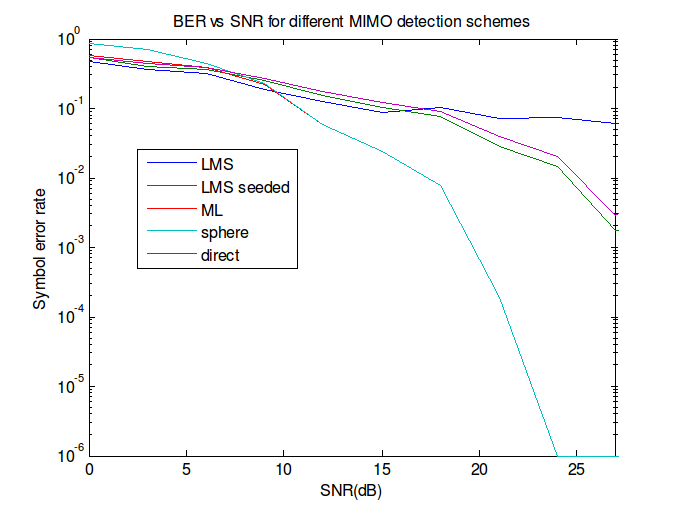
\includegraphics[width=8cm]{images/static_channel_decoder_comparison.png}
\caption{SER vs SNR for different MIMO detection schemes with a static channel}
\label{ser_snr_different_schemes_static}
\end{figure}

\begin{figure}
\centering
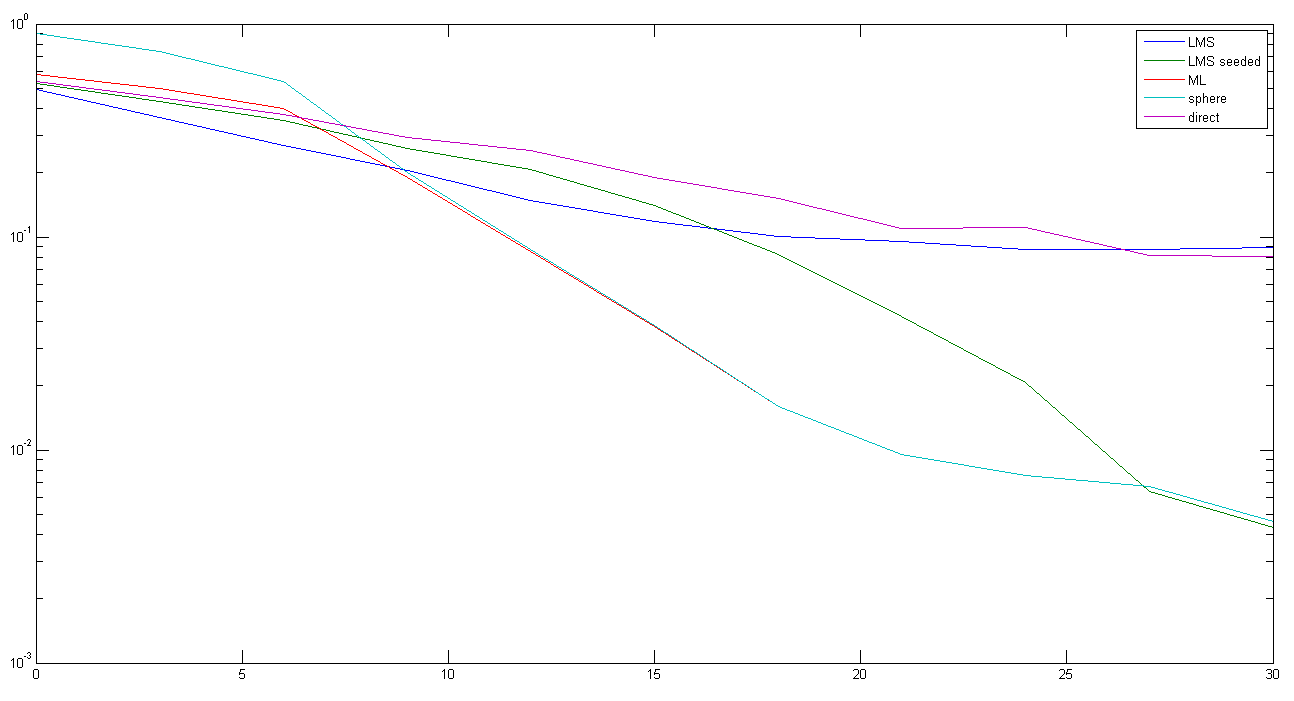
\includegraphics[width=9cm]{images/time_varying_channel_doppler_3.png}
\caption{SER vs SNR for different MIMO detection schemes with a time varying channel (doppler shift of 3Hz)}
\label{ser_snr_different_schemes_dynamic}
\end{figure}

Adaptation can be combined with the MMSE linear detection scheme into the following algorithm:
\begin{enumerate}
\item Estimate the channel matrix based on {\em a prior} known training sequence.
\item Compute initial MMSE receive filter
\item Begin processing received samples using receive filter matrix.
\item Adapt receive filter using LMS algorithm to track channel variations.
\end{enumerate}

We implemented an LMS-MMSE MIMO decoder since this has relatively low implementation complexity but can show the usefulness of this technique and is easily extendable to more complicated receive processing. For example, MMSE-SIC detection can be accomplished by adaptively estimating the channel and performing the decoding one stream at a time instead of simultaneously. 

%%%% ARCHITECTURE SECTION %%%%
\section{Hardware Architecture}

The archictecture of the Adaptive MIMO Decoder is shown in Figure~\ref{top_level_arch}. The host configures the decoder by writing to the configuration registers, setting up the number of antennas used, the length of the training sequence, the modulation scheme used and the current SNR. Since different standards use different training sequences, the host then needs to write the current training sequence to the training memory. Once complete, the host writes a 1 to the {\em start} register, and begins sending samples to the RX Data Queue.

The Channel Estimator uses the training sequence and the first few received samples to estimate the channel matrix H. This channel matrix is then sent to the Initialize Weights module, which computes the initial decoder matrix W\_seed. The Adaptive Decoder uses this W\_seed as a starting point for its decoder matrix W. The Adaptive Decoder decodes the samples in the RX Data Queue and writes the decoded symbols to the Decoded Data Queue. For each set of samples, the Adaptive Decoder also updates the W matrix.

Finally, the host reads the decoded symbols from the Decoded Data Queue. Each of the different modules in the design will now be described in more detail below.

\begin{figure}[!h]
\centering
\includegraphics*[width=9cm, viewport = 0 90 789 600]{images/top_level_arch.pdf}
\caption{The hardware architecture of the LMS Adaptive MIMO Decoder}
\label{top_level_arch}
\end{figure}

\subsection{Matrix Engine}

The Matrix Engine computes the complex vector-matrix multiply between an input vector V and an input matrix M. The input matrix M has size (number transmit antennas) x (number receive antennas). Since the Adaptive Decoder needs to decode a new set of antenna samples every cycle, the Matrix Engine needs to compute the vector-matrix multiply in a single cycle. For the 4x4 MIMO case, it does this using four dot-product units (each of which compute the dot product between two 4-element vectors) which operate in parallel. However, if only 2x2 MIMO needs to be supported, then only two dot-product units will be created at compile time.

\begin{figure}[!h]
\centering
\includegraphics*[width=4cm, viewport = 30 640 260 840]{images/matrix_engine.pdf}
\caption{Design of the matrix engine}
\label{matrix_engine}
\end{figure}

\subsection{Channel Estimator Module}

The channel estimator module uses the known training sequence as well as the corresponding received symbols to compute the initial channel estimate. We have used a training sequence which is orthogonal in space and time, mimicking the general format of the 802.11ac VHT-LTF fields but not the specifics. Since the training sequence is an orthogonal matrix, the channel estimate can be obtained simply from a matrix multiplication of the training sequence matrix with the received signals matrix. The channel estimator module uses the matrix engine to perform this computation and then sends the result to the weight initialization module.

\subsection{Initialize Weights Module}

The initialize weigts module computes the MMSE receive filter using the initial channel estimate, H:
\[W = (H^H H + \sigma^2I)^{-1} H^H \]

The main operations required are two matrix multiplications and one matrix inversion. The matrix multiplications are performed using the matrix engine, while a specialized 2x2 matrix inversion hardware is contained within this module. For 2x2 MIMO cases it is sufficient to simply use this module, while for larger MIMO orders the matrix is inverted blockwise using the 2x2 matrix inversion engine and small additional hardware.

\subsubsection{2x2 Matrix Inversion}

For 2x2 matrices, the inverse can be computed efficiently using the explicit formula:
\[\left[ \begin{array}{cc} x_{11} & x_{12} \\ x_{21} & x_{22} \end{array}\right]^{-1} = \frac{1}{x_{11}x_{22}-x_{12}x_{21}}\left[ \begin{array}{cc} x_{22} & -x_{12} \\ -x_{21} & x_{11} \end{array}\right]\]

This calls for two complex multiplications and a subtraction (to compute the determinant) and four complex divisions. Since the complex division requires a large and power-hungry hardware, we use a single complex divider (pipelined in three stages) which is multiplexed to perform the four divisions per 2x2 matrix. Thus, inversion of a 2x2 matrix takes 13 cycles (including one for determinant computation).

\subsubsection{Inversion of Larger Matrices}

To invert larger matrices, the 2x2 matrix inversion hardware and the matrix engine are used. The inversion is performed blockwise:
\[\left[ \begin{array}{cc} A & B \\ C & D \end{array}\right]^{-1} = \left[ \begin{array}{c} A^{-1}+A^{-1}B(D-CA^{-1}B)^{-1}CA^{-1} \\ -(D-CA^{-1}B)^{-1}CA^{-1} \end{array} \right] \]
\[ \left[ \begin{array}{c} -A^{-1}B(D-CA^{-1}B)^{-1} \\  (D-CA^{-1}B)^{-1} \end{array}\right]\]

NEED TO FIX EQUATION TO USE MULTILNE

For a 4x4 matrix inversion, this requires two 2x2 matrix inversions as well as several 2x2 matrix multiplications, which are performed using their respective dedicated hardware. We currently have not implemented 3x3 matrix inversion, but it can accomplished with minimal hardware overhead by using this same approach. 

\begin{figure}
\centering
\includegraphics*[width=8cm]{images/initialize_weights.jpg}
\caption{Weight initialization module}
\label{initialize_weights}
\end{figure}

\subsection{Adaptive Decoder Module}

The task of the Adaptive Decoder Module is simply to decode the samples received from the antennas into the symbols for the independent data streams. It does this by multiplying the received samples (vector $v$) with the decoder matrix $W$, using the Matrix Engine. This is shown in Figure~\ref{adaptive_decoder}. The $Wx$ vector is then converted into a vector of symbols $y$ using a simple slicer to find the nearest constellation points. The $error$ between $Wx$ and the decoded symbols is computed and multiplied by a step-size parameter $\mu$.

This weighted error is used to update the decoder matrix according to the following equation:
\[ W_{next} = W - x \times (error \cdot \mu) \]

Note that $x \times (error \cdot \mu)$ is the vector cross-product between received samples $x$ and the error weighted by $\mu$.
\begin{figure}[!h]
\centering
\includegraphics*[width=8cm, viewport = 0 510 560 810]{images/adaptive_decoder.pdf}
\caption{The adaptive decoder module}
\label{adaptive_decoder}
\end{figure}

\subsection{Evaluation of Bitwidths}

The LMS MIMO Decoder architecture described above was implemented in Chisel \cite{chisel}. In order to verify correctness and determine the optimum bitwidths to use, the design was tested in Chisel, using test vectors taken from the MATLAB simulations (as described in Section \ref{matlab_comparison_section}). The symbol error rate versus SNR plots for different bitwidths, for a static channel, are shown in Figure~\ref{ser_ber_chisel_static}. This plot also includes the results from the MATLAB simulation for comparison. Similarly, Figure~\ref{ser_ber_chisel_dynamic} shows the SER vs SNR plots for a slowly changing channel.

\begin{figure}[!h]
\centering
\includegraphics*[width=8cm, viewport = 80 260 560 530]{images/snr_ber_curves_chisel_static.pdf}
\caption{SER vs SNR curves for Chisel implementations with different bitwidths (static channel)}
\label{ser_ber_chisel_static}
\end{figure}

\begin{figure}[!h]
\centering
\includegraphics*[width=9cm, viewport = 80 270 560 530]{images/snr_ber_curves_chisel_doppler.pdf}
\caption{SER vs SNR curves for Chisel implementations with different bitwidths (dynamic channel)}
\label{ser_ber_chisel_dynamic}
\end{figure}

For the static channel, the 20 bit and 24 bit Chisel implementations very closely track the MATLAB simulations, while the 16 bit simulation is completely incorrect. However, for the dynamic channel, where higher precision is needed to track the changing channel, only the 24 bit implementation is able to match the performance of the MATLAB simulation. Therefore, 24 bits was selected as the desired bitwidth for the design.

The poor performance at lower bitwidths is caused by arithmetic overflow during the matrix inverse operation in the Initialize Weights module. Since the channel matrix H can be poorly conditioned, the entries in its inverse matrix can have a high dynamic range, resulting in arithmetic overflow if too few bits are used. Better performance can be achieved at lower bitwidths if saturating arithmetic or pseudo-floating-point were used. Unfortunately, neither of these two features are currently supported in Chisel.


%%%% SYNTHESIS CONSTRAINTS SECTION %%%%
\section{Synthesis Options and Constraints}

The clock rate at which the design was synthesized was determined by maximum throughput requirements for 802.11ac and LTE. When utilizing an 80MHz channel, 802.11ac base stations can transmit 278 000 symbols/sub-carrier/antenna/second \cite{802_11_ac_handbook}. With 234 sub-carriers, this translates to 70 million symbols/second/antenna.

LTE, on the other hand, has a maximum symbol rate of only 14 000 symbols/sub-carrier/antenna/second, but with 1200 sub-carriers \cite{lte_webpage}. This results in a throughput of 16.8 million symbols/second/antenna.

If the sub-carriers are decoded sequentially at the receiver (i.e. multiplexing the decoder between the sub-carriers, in time), but all the antenna streams are decoded in parallel, the Adaptive MIMO Decoder will therefore need to be clocked at 70MHz (i.e. at the symbols/antenna rate). However, it is possible to process multiple sub-carriers in parallel, as each sub-carrier is completely independent of the others. The advantage of this approach is that all the sub-carriers can share (on a time-multiplexing basis) common Channel Estimation and Weight Initialization modules, as these modules only run for a short period of time at startup. The only modules that therefore need to be duplicated are the the Matrix Engine and the Adaptive Decoder.

Table~\ref{clock_rate_table} therefore shows the required clock rate for parallelism levels of 1, 2 and 4. Note that the level of parallelism indicates both the number of sub-carriers that can be decoded in parallel, as well as the number of instantiations of the Matrix Engine and Adaptive Decoder. This means that all three scenarios shown in the table have {\em identical} throughput.

\begin{table}[!h]
\caption{VLSI clock rate for different levels of parallelism}
\label{clock_rate_table}
\centering
\begin{tabular}{l l}
\hline
Number of parallel sub-carriers & Clock Rate \\
\hline
1 & 70 MHz \\
2 & 35 MHz \\
4 & 17.5 MHz \\
\hline
\end{tabular}
\end{table}

While estimating the channel matrix at the beginning of each packet (using the Long Training Field in the 802.11ac PHY header) and computing the resulting (initial) weight matrix does take time, special care was taken to ensure that this will not impact the latency and throughput requirements of 802.11ac and LTE. Since these initialization operations only take 50 clock cycles, but decoding entire packet takes 45000 cycles (or more, if aggregate packets are used), the initialization delay is easily handled by performing a small amount of buffering in the input queues and increasing the clock rate by 1-2\%.


%%%% SYNTHESIS RESULTS SECTION %%%%
\section{Synthesis Results}

The Chisel designed was synthesized at the three clock rates shown in Table~\ref{clock_rate_table}. Note that for the 35 MHz and 17.5 MHz cases, the Matrix Engine and Adaptive Decoder modules were replicated the required number of times. The results are shown in Figure~\ref{power_vs_area}, for a 4 antenna decoder. Again, it must be emphasized that all three synthesized versions have the same throughput, and are able to meet the requirements for 802.11ac and LTE.

\begin{figure}[!h]
\centering
\includegraphics*[width=8cm, viewport = 60 250 560 540]{images/power_vs_area.pdf}
\caption{Power vs area for different levels of parallelism}
\label{power_vs_area}
\end{figure}

It is quite clear that the 24-bit 70MHz version results in the smallest area (0.6mm$^2$) and lowest power (78mW). While the 20-bit version does result in a slightly smaller design, it cannot be used due to poor reliability in changing channel conditions (as previously explained). Lower power figures at the slower clock rates could probably be achieved if voltage scaling was used; however, this feature was not available to us.

Furthermore, extrapolating from Figure~\ref{power_vs_area} shows that even smaller area/power figures could be obtained if the data streams from the 4 antennas were processed sequentially (rather than in parallel, as they are currently done), and the clock rate was increased accordingly.

The power consumed by each module in the MIMO decoder is shown in Table~\ref{power_breakdown_table} and illustrated in Figure~\ref{power_breakdown_module}. These show that almost half the power (35.8mW) is consumed by the initialization modules: Channel Estimator and Initialize Weights. Since these modules are only used for a very short period of time at the beginning of each packet ($<$ 0.1\% of the time), power gating them will reduce the average power consumption to 42mW.

\begin{table}[!h]
\caption{Breakdown of power by module}
\label{power_breakdown_table}
\centering
\begin{tabular}{l l l r}
\hline
Module & Submodule & & Power (mW) \\
\hline
Channel Estimator & & & 2.13 \\
Initialize Weights & Mat4 Inverse & 3.96 & \\
 & Mat2 Inverse & 24.8 & \\
 & Module total & & 33.7 \\
Matrix Engine & & & 25.4 \\
Adaptive Decoder & & & 15.1 \\
Queues & & & 1.81 \\
\hline
\em{Total} & & & \em{78.14} \\
Total without & & & \\
initialization modules & & & 42.31 \\
\hline
\end{tabular}
\end{table}

\begin{figure}[!h]
\centering
\includegraphics*[width=6cm, viewport = 90 100 660 540]{images/power_breakdown_module.pdf}
\caption{Power of LMS MIMO Decoder by module}
\label{power_breakdown_module}
\end{figure}

ANTONIO: if you can, please insert some 2x2 vs 4x4 results here. Mention that 4x4 hardware supports 2x2, but more efficient to generate 2x2 hardware.

ANTONIO: do we want to compare to area/power of other MIMO decoders from the literature?


%%%% CONCLUSION AND FUTURE WORK SECTION %%%%
\section{Conclusions and Future Work}

In this project, we have demonstrated an adaptive LMS-MMSE MIMO decoder that can achieve the throughput requirements of LTE and 802.11ac using QPSK modulation. The final design takes up less than 0.5 $mm^2$ of area and consumes 42mW when including power gating of the initialization blocks. By exploiting the LMS adaptive loop, this design is also able to track slow channel variations while maintaining good performance.

There are several areas of further work that could improve this design:
\begin{enumerate}
\item Implement a real control loop to turn off the initialization modules when they are not in use.
\item Optimize the bit-widths to reduce area and power. Probably it is sufficient to keep longer bit widths in the initialization block (where the matrix inversion is sensitive to precision errors) and reduce the bit widths in the main adaptive decoder. The required bit width in the inversion block could also be reduced by using pseudo-floating point or saturating arithmetic.
\item Evaluate energy reduction techniques when using parallel processing modules. Since each module can operate with a lower throughput, it should be possible to reduce energy per decoded symbol by reducing the supply voltage.
\item Design a control loop to dynamically select the LMS step size based on the time scale of channel variations.
\item Integrate this MIMO receiver with a channel decoder and use the decoder hard decisions to adapt the receive filter.
\end{enumerate}


% references section

\bibliographystyle{IEEEtran}
\bibliography{refs}

\end{document}


